\section{The New Patch Collection Process}
\begin{frame}
  \frametitle{The Final Patch Collection Process}
  \begin{figure}
    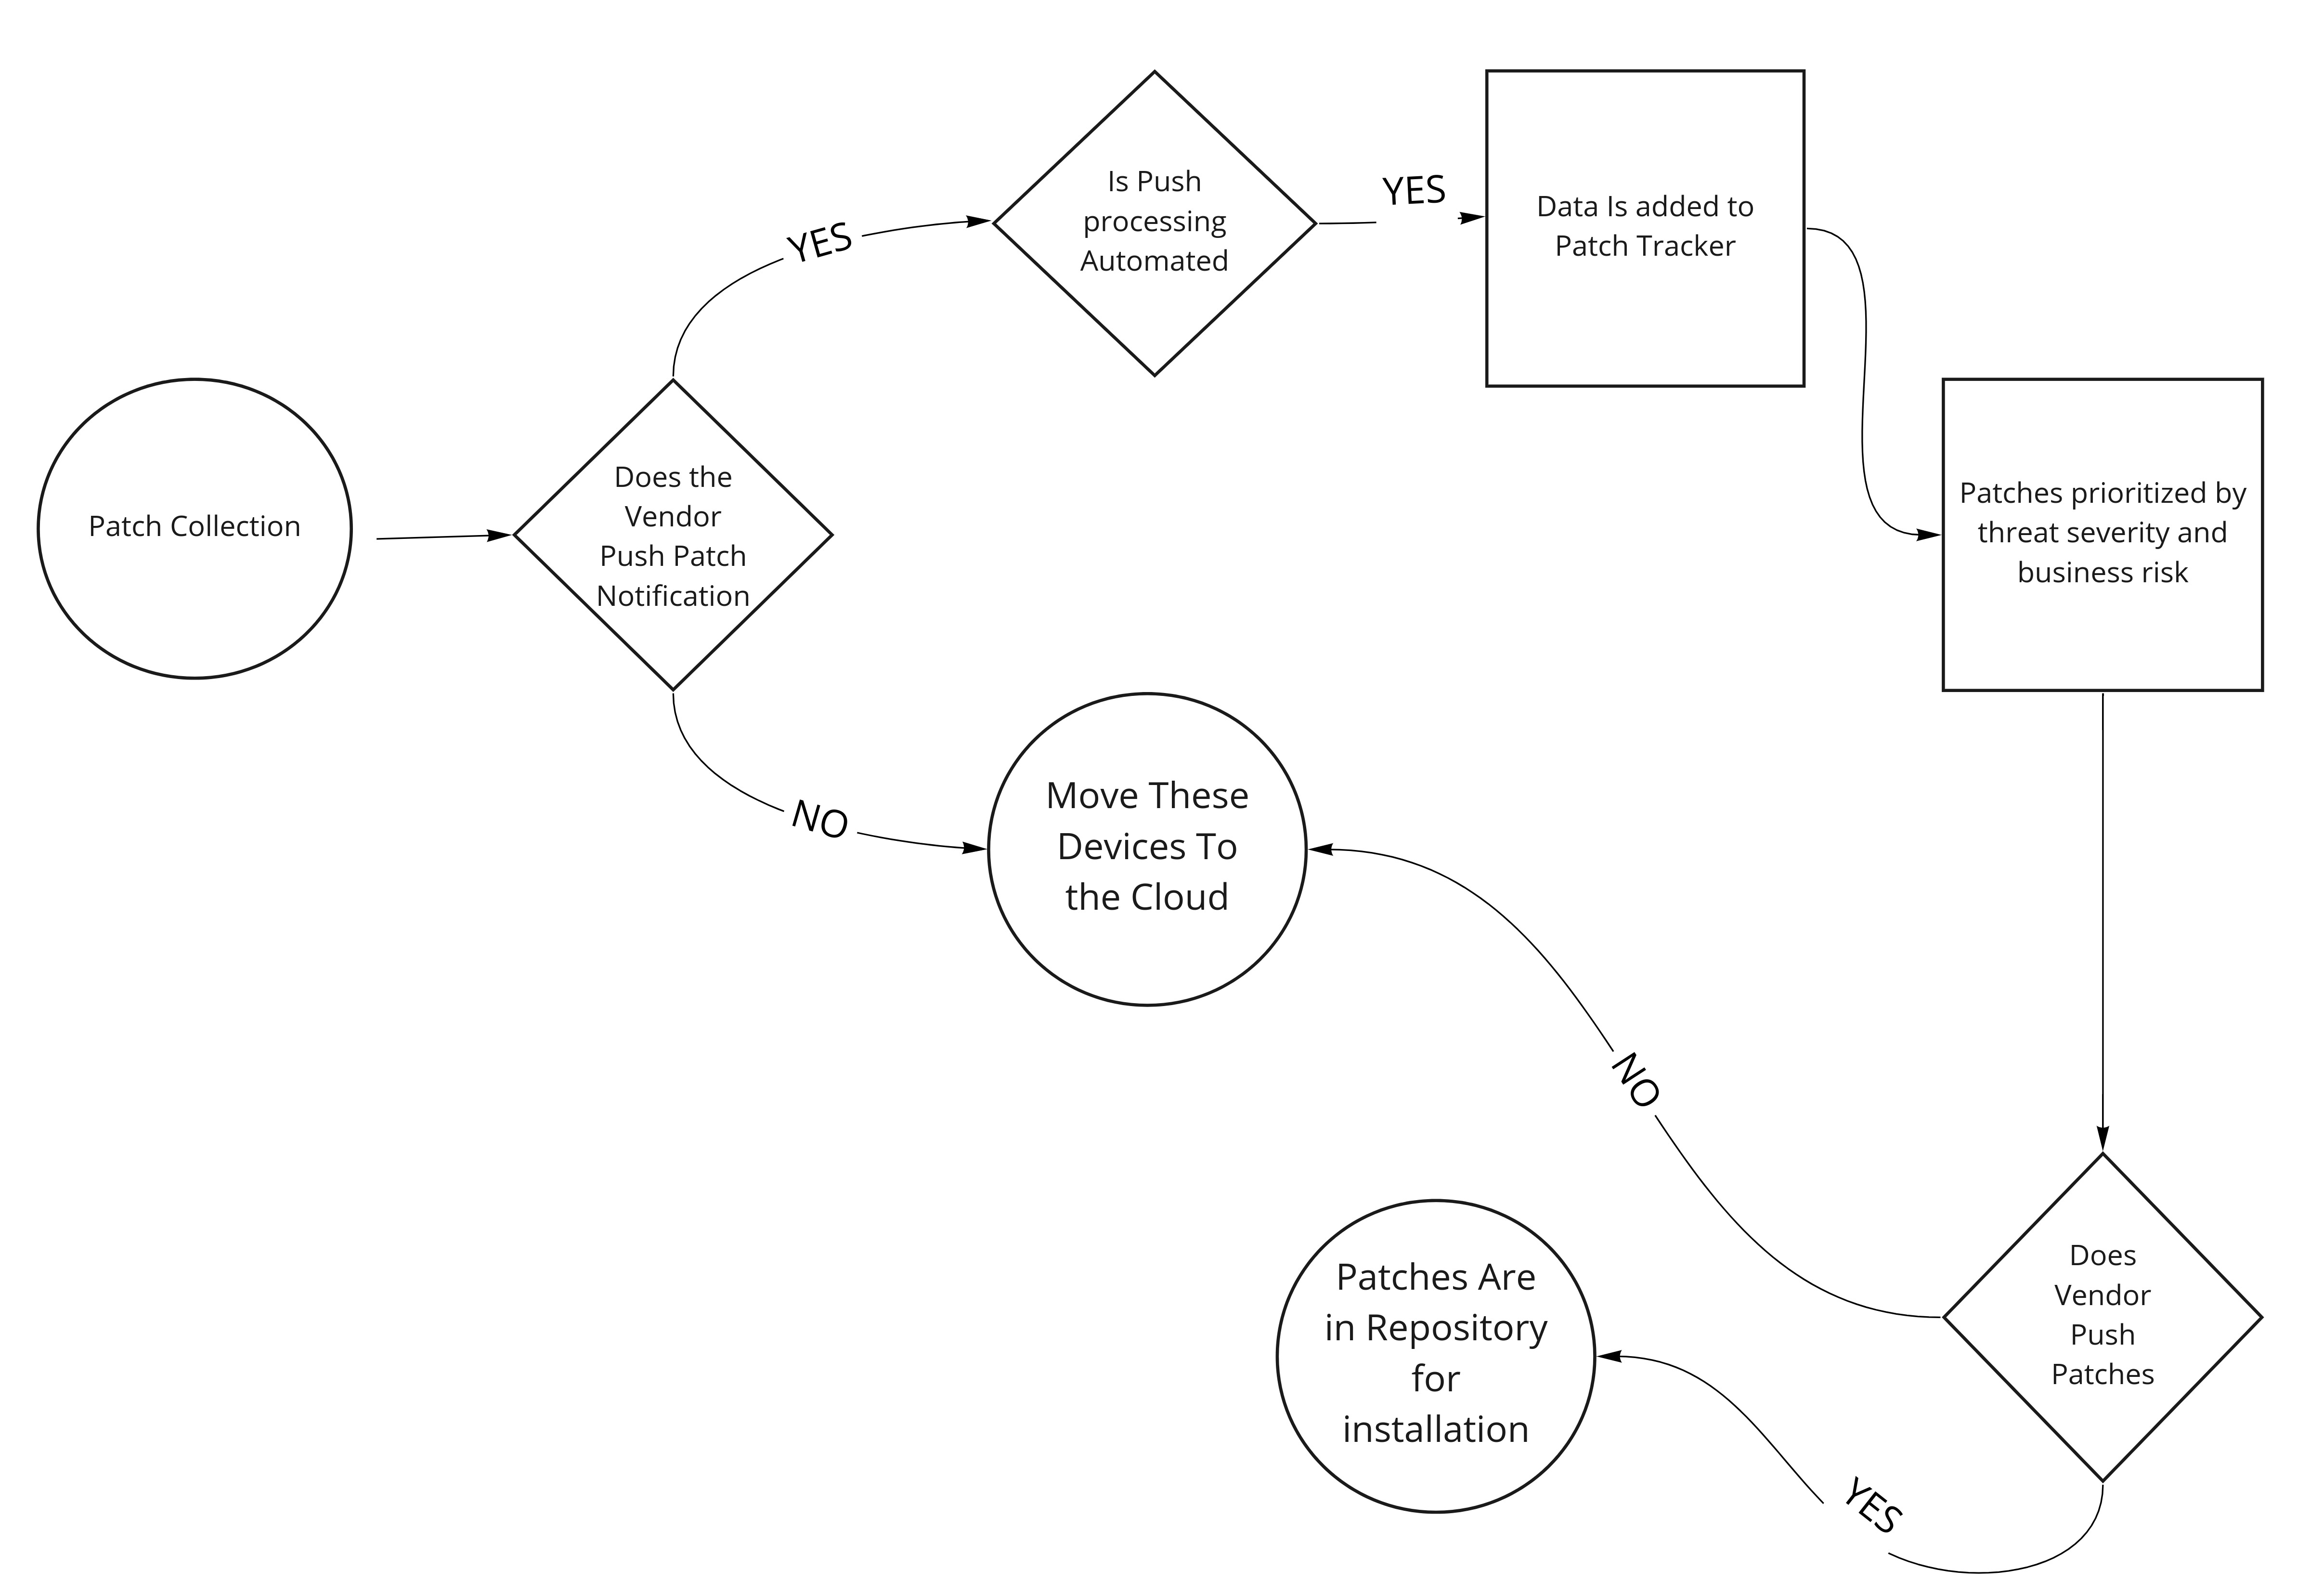
\includegraphics[width=0.8\textwidth]{img/final}
\end{figure}

\note[item]{\scriptsize{All devices that lack automation from the vendor side must be targeted for being moved to an IaaS solution in the cloud. In the interim period between now and the achievement of this goal, the previously defined manual steps will have to be maintained or automated. While it is the recommendation to automate those steps, it is understood that management concern for legal liability may preclude this automation from being approved. Ultimately, however, the end-state should not allow for un-automated security tracking for infrastructure services that are not in the cloud.}}

\note[item]{\scriptsize{Devices that do have automated systems for pushing out patch data and patches themselves should also be included in moves to the cloud for other operational cost reduction reasons. However, there is no benefit to this process in doing so. As such, these systems should not be included in the project, as they are already in a fully automated process.}}


\end{frame}
